% chktex-file 1
% chktex-file 2
% chktex-file 3
% chktex-file 8
% chktex-file 9
% chktex-file 12
% chktex-file 13
% chktex-file 16
% chktex-file 18
% chktex-file 24
% chktex-file 26
% chktex-file 35
% chktex-file 44
% chktex-file 45
\documentclass[]{article}
\usepackage[utf8]{inputenc}
\usepackage[english]{babel}

\usepackage[]{csvsimple}
\usepackage{float}

\usepackage{ragged2e}
\usepackage[left=25mm, right=25mm, top=15mm]{geometry}
\geometry{a4paper}
\usepackage{graphicx}
\usepackage{booktabs}
\usepackage{paralist}
\usepackage{subfig} 
\usepackage{fancyhdr}
\usepackage{amsmath}
\usepackage{amssymb}
\usepackage{amsfonts}
\usepackage{amsthm}
\usepackage{mathtools}
\usepackage{enumitem}
\usepackage{titlesec}
\usepackage{braket}
\usepackage{gensymb}
\usepackage{url}
\usepackage{hyperref}
\usepackage{csquotes}
\usepackage{multicol}
\usepackage{graphicx}
\usepackage{wrapfig}
\usepackage{babel}
\usepackage{caption}
\captionsetup{font=small}
\pagestyle{fancy}
\renewcommand{\headrulewidth}{0pt}
\lhead{}\chead{}\rhead{}
\lfoot{}\cfoot{\thepage}\rfoot{}
\usepackage{sectsty}
\usepackage[nottoc,notlof,notlot]{tocbibind}
\usepackage[titles,subfigure]{tocloft}
\renewcommand{\cftsecfont}{\rmfamily\mdseries\upshape}
\renewcommand{\cftsecpagefont}{\rmfamily\mdseries\upshape}

\let\oldsection\section% Store \section
\renewcommand{\section}{% Update \section
	\renewcommand{\theequation}{\thesection.\arabic{equation}}% Update equation number
	\oldsection}% Regular \section
\let\oldsubsection\subsection% Store \subsection
\renewcommand{\subsection}{% Update \subsection
	\renewcommand{\theequation}{\thesubsection.\arabic{equation}}% Update equation number
	\oldsubsection}% Regular \subsection

\newcommand{\abs}[1]{\left\lvert#1\right\rvert}
\newcommand{\norm}[1]{\left\lVert#1\right\rVert}

\newcommand{\g}{\text{g}}
\newcommand{\m}{\text{m}}
\newcommand{\cm}{\text{cm}}
\newcommand{\mm}{\text{mm}}
\newcommand{\s}{\text{s}}
\newcommand{\N}{\text{N}}
\newcommand{\Hz}{\text{Hz}}

\newcommand{\virgolette}[1]{``\text{#1}"}
\newcommand{\tildetext}{\raise.17ex\hbox{$\scriptstyle\mathtt{\sim}$}}


\renewcommand{\arraystretch}{1.2}

\addto\captionsenglish{\renewcommand{\figurename}{Fig.}}
\addto\captionsenglish{\renewcommand{\tablename}{Tab.}}

\DeclareCaptionLabelFormat{andtable}{#1~#2  \&  \tablename~\thetable}


\title{%
    \Huge Misura della carica dell'elettrone \\
    \Large Laboratorio di Ottica, Elettronica e Fisica Moderna \\ C.d.L. in Fisica, a.a. 2023-2024 \\ Università degli Studi di Milano}
\author{\LARGE Lucrezia Bioni, Leonardo Cerasi, Giulia Federica Bianca Coppi \\ Matricole: 13655A, 11410A, 11823A}
\date{26 ottobre 2023}

\begin{document}

    \maketitle

    \section{Introduzione}
    \subsection{Scopo}
    Utilizzando l'apparato sperimentale di Millikan, si vuole misurare la carica elementare dell'elettrone. Tale grandezza viene ottenuta mediante la misurazione della velocità di sedimentazione delle gocce elettricamente cariche all'interno dell'apparato.

    \subsection{Metodo}
    All'interno della camera di Millikan, vengono spruzzate delle goccioline di olio che - elettrificate a causa dello strofinio con altre goccioline - si muovono di moto rettilineo uniforme, sia in assenza che in presenza di un campo elettrico esterno $E$. \\ La descrizione del moto delle goccioline è dato alle seguenti equazioni, rispettivamente in assenza e in presenza di campo elettrico: 
    \begin{equation}
        \label{moto1}
        \frac{4 \pi}{3} r^3 (\rho_o - \rho_a) g - 6 \pi \eta r v_o = 0
    \end{equation}
        
    \begin{equation}
        \label{moto2}
        \frac{4 \pi}{3} r^3 (\rho_o - \rho_a) g - 6 \pi \eta r v_o + qE= 0
    \end{equation}

    dove r è il raggio della goccia, $\rho_o $ la densità della goccia di olio, $ \rho_a$ la densità dell'aria, $g$ l'accelerazione di gravità, $\eta$ la viscosità dell'aria, $v_o$ la velocità limite in assenza di campo elettrico $E$ e $v$ la velocità limite in presenza del campo elettrico $E$.\\
    La carica goccia presa in esame viene determinata attraverso un'ulteriore analisi qualitativa riguardante il verso del suo moto: quando la goccia scende prevalgono forze dirette verso il basso, mentre quando sale prevalgono forze dirette verso l'alto. Si può ricavare la seguente espressione per la carica della goccia:
    \begin{equation}
        \label{carica-def}
        q= - \frac{4 \pi}{3} r^3 (\rho_o - \rho_a) \frac{g}{E} \left( 1 - \frac{v}{v_o} \right)
    \end{equation}

    Dunque la determinazione della carica della goccioliina d'olio elettrificata richiede la misura della sua velocità limite nelle tre situazioni ($E=0$, $v<0$, $v>0$) e del suo raggio. Quest'ultima grandezza influenza la viscosità effettiva dell'aria secondo la relazione studiata da Millikan
    \begin{equation}
        \label{eta_eff}
        \eta_{\text{eff}}=\frac{\eta}{1 + \frac{b}{p r}}
    \end{equation}
    dove $\displaystyle \eta = \left[1.800 + (T -15)4.765 \cdot 10^{-3} \right] \cdot 10^{-5} \,\text{N s m}^{-2}$ è la viscosità dell'aria, $t$ è la temperatura (in gradi Celsius), $p$ la pressione dell'aria presente nella camera di Millikan e $b$ una costante dei gas che per l'aria vale $b=8.2 \cdot 10^{-3} \, \text{Pa m}$.\\ Si ricava quindi che il raggio della gocciolina di olio è 
    \begin{equation}
        \label{raggio-def}
        r=\sqrt{\left( \frac{b}{2p} \right) ^2 + \frac{9 \eta v_o}{2 g \left(\rho_o - \rho_a \right)}} - \frac{b}{2p}
    \end{equation}


    \section{Misure}

    \subsection{Misure preliminari}
    \label{par:misure-preliminari}

    Innanzi tutto si prendono 6 misure - mediante l'utilizzo di un calibro di sensibilità $ 0.01\, mm $ - dello spessore $ d $ del disantaziale della camera di Millikan

    \begin{table}[H]
        \centering
    
        \begin{tabular}{||c||}
            \hline
            $d\, \text{[mm]} $ \\
            \hline\hline
    
            $ 7,65 $ \\\hline
            $ 7,64 $ \\\hline
            $ 7,63 $ \\\hline
            $ 7,64 $ \\\hline
            $ 7,64 $ \\\hline
            $ 7,63 $ \\\hline

        
        \end{tabular}
        \caption{Misure dello spessore del distanziale}
        \label{distanziale}
    \end{table}

    Viene quindi attribuito come valore finale a $ d $ la sua media con la relativa incertezza strumentale:

    \begin{equation}
        \label{misura_Rb}
        d = (7.64 \pm 0.01) \, \text{mm}
    \end{equation} 
    Per ciascun set di misure, si è misurata la temperatura della cameretta in cui avviene il moto delle gocce di olio. In particolare, mediante multitmetro, si è misurata la resistenza elettrica di un termistore. Attraverso una apposita tabella di conversione, poi, si è determinato il valore della temperatura sulla base di quello della resistenza. L'incertezza attribuita alla temperatura è la semiampiezza del minimo intervallo risolubile dalla tabella utilizzata, ovvero $5 \degree \text{C}$.
    La temperatura relativa a ciascuna goccia è riportata nella caption della tabella ad essa corrispondente in Appendice.

    \subsection {Costanti}
    \label{par:costanti}

    Le seguenti quantità, che saranno necessarie per la determinazione della grandezza in esame, vengno assunte costanti:
    \begin{itemize}
        \item accelerazione di gravità $g = 9.806 \, \text{m s}^{-2}$;
        \item densità dell'olio $\rho_o = 860 \, \text{kg m}^{-3}$;
        \item densità dell'aria $\rho_a = 1.293 \, \text{kg m}^{-3}$;
        \item pressione atmosferica $ p = 101325 \, \text{Pa}$;
        \item costante legata alla viscosità dell'aria $b = 0.0082 \,  \text{Pa m}$;
        \item distanza delle righe del reticolo $ \Delta z = 0.5 \, \text{mm}$;
    \end{itemize}

    \subsection {Misure effettive}
    Si scelgono 10 gocce di cui registrare il moto nelle due condizioni: in assenza e in presenza di campo elettrico $ E $. In presenza del campo, a seconda del segno della forza elettrica agente sulla goccia $F_e = qE$, si osserva, attraverso microscopio, un moto ascendente o discendente. Si misura quindi la differenza di potenziale applicata e il tempo che ogni goccia impiega a percorrere $ \Delta z = 0.5 \, \text{mm} $. La porzione di spazio percorsa viene considerata priva di errore. A tali grandezze si corredano ulteriori informazioni: il verso del moto - se sale o se scende - e dati qualitativi come eventuale presenza di rumore e comportamenti anomali. \\
    Tutti i dati vegono riporati nelle tabelle in Appendice. \\ 
    La misura del tempo di volo è stata effetuata mediante un cronometro digitale di risuluzione $ 0.01 \, \text{s} $. La misurazione della differenza di potenziale $ \Delta V $ è stata effettuata mediante un multimetro digitale a cui viene attribuita come incertezza $ 1 \, \text{V} $.


    \section{Analisi Dati}
    \subsection{Misura del raggio delle gocce}
    Nella configurazione di assenza di campo, si determina il raggio delle gocce di olio osservate.
    Una volta raggiunta la velocità limite nel mezzo $v_0$, il moto della goccia risulta essere rettilineo uniforme. Dunque, dallo studio del moto della goccia, si determina la sua velocità di caduta, cui si attribuisce incertezza mediante propagazione degli errori sull'intervallo di tempo $t$. I valori di velocità così ottenuti sono riportati nelle tabelle in Appendice.

    Ai fini della determinazione del raggio della goccia, è inoltre necessario stimare il coefficiente di viscosità del mezzo:
    \begin{equation}
        \label{viscosita}
        \eta(T) = \left[ 1.800 + 4.765 \cdot 10^{-3} \, \degree \text{C}^{-1} \left( T - 15 \degree \text{C} \right) \right] 10^{-5} \,\text{N s m}^{-2}  
    \end{equation}
    A tale valore è stata attribuita un'incertezza mediante propagazione degli errori:
    \begin{equation}
        \label{sigma-eta}
        \sigma_{\eta}= 4.765 \cdot 10^{-8} \text{N s m}^{-2}
    \end{equation}
    Grazie ai valori di $\eta$ e di $v_0$ ottenuti è possibile determinare il raggio di ciascuna goccia attraverso la seguente relazione:
    \begin{equation}
        \label{raggio}
        r = \sqrt{\left( \frac{b}{2p} \right)^2 + \frac{9 \eta v_0}{2g \left( \rho_{o} - \rho_a\right)}} - \frac{b}{2p}
    \end{equation}
    dove $p$, $g$, $\rho_o$ e $\rho_a$ sono costanti riportate in Par. \ref{par:costanti}, $b$ è un parametro empirico per correggere $\eta$, pari a $8.2 \cdot 10^{-3} \text{Pa m}$. Tale correzione è necessaria poiché il libero cammino medio di una molecola di aria, dell'ordine di $10^{-6} \text{m}$, è confrontabile con il raggio delle gocce di olio osservate al microscopio, dell'ordine di $10^{-7} \text{m}$.
    A ciascun valore di raggio $r$ è stata attribuita incertezza mediante propagazione degli errori sulle grandezze $t$ ed $T$, la cui dipendenza è situata in $v_0$ ed $\eta$:
    \begin{equation}
        \sigma_r= \frac{9 \eta}{ 4 g \Delta t \left(\rho_o - \rho_a \right) \left(r+\frac{b}{2p} \right)} \sqrt{ \left(v \sigma_t\right)^2 + \left( \frac{\Delta z}{\eta} \sigma_{\eta} \sigma_T \right)^2}
    \end{equation}
    I valori ottenuti sono riportati nelle tabelle in Appendice.

    \subsection{Misura della carica delle gocce}
    \label{par:cariche-olio}
    In presenza di campo elettrico $E = \frac{\Delta V}{d}$, si determina la velocità $v_E$ limite delle medesime gocce di cui si è determinato il raggio $r$, attraverso la relazione per un moto rettilineo uniforme, cui si attribuisce un segno in base al verso del moto (positivo se verso il basso, negativo se verso l'alto). A tali valori di velocità è stata attribuita incertezza mediante propagazione degli errori sulla grandezza $t$. \\
    Le misure effettuate sono riportate nelle tabelle in Appendice.
    
    Si determina poi la carica $Q$ di ciascuna goccia di olio attraverso la seguente relazione:
    \begin{equation}
        \label{Q}
        Q = -\frac{4}{3} \pi r^3 \left( \rho_o - \rho_a \right) \frac{g d}{\Delta V} \left( 1 - \frac{v_E}{v_r} \right)
    \end{equation}
    dove $r$ è il raggio della goccia osservata precedentemente determinato, $v_E$ è la velocità limite della goccia in presenza di campo elettrico $E$ e $v_r$ è la media delle velocità limite della goccia registrate in assenza di campo elettrico.
    I valori così calcolati sono riportati nelle tabelle in Appendice. 
    Poiché si è osservato che alcuni valori di carica $Q_i$ non sono compatibili con gli altri relativi alla medesima goccia, e poiché si è osservato che alcune gocce presentano tempi di acquisizione sotto campo molto brevi (inferiori ai $2s$), si è provato a rigettare tali dati (contrassegnati da asterisco $\ast$ nelle tabelle in Appendice), e a effettuare l'analisi del dataset scremato. Tuttavia, si è osservato che il valore di carica elettronica $q_e$ così ottenuto è meno compatibile con il valore atteso rispetto a quello ottenuto con il dataset completo. Pertanto, si è deciso di proseguire l'analisi con il dataset completo. Si riportano, nella seguente tabella, i risultati ottenuti:

    \begin{table}[H]
        \centering
    
        \begin{tabular}{|| c || c | c||}
            \hline
            $ $ & $q_e \pm \sigma_{q}\, \cdot 10^-{19} \text{[C]} $ & $ (q_e - e)/e$\\
            \hline\hline
    
            $\text{dataset completo}$ & $ 1.57 \pm 0.01 $ & $1.83 \%$\\\hline
            $\text{dataset scremato}$ & $ 1.45 \pm 0.06 $ & $9.29 \%$ \\\hline
        \end{tabular}
        \caption{Valori della carica elettronica, con rispettiva incertezza e distanza percentuale dal valore atteso, ottenuti con il dataset completo e scremato.}
        \label{carica-eletronica}
    \end{table}

    L'incertezza associata a ciascuna misura di $Q$ è stata determinata mediante propagazione degli errori nella \ref{Q} sulle grandezze $r$, $d$, $\Delta V$ e $v_r$. L'incertezza su $v_r$ è stata attribuita mediante deviazione standard.
    \begin{equation}
        \label{sigma-Q}
        \sigma_Q = \abs{Q} \sqrt{ \left( 3 \frac{\sigma_r}{r} \right)^2 + \left( \frac{\sigma_d}{d} \right)^2 + \left( \frac{\sigma_{\Delta V}}{\Delta V} \right)^2 + \frac{1}{\left( v_r - v_E \right)^2}\left( \frac{v_E}{v_r} \sigma_{v_r} \right)^2 }
    \end{equation}
    Non si è propagato l'errore relativo agli intervalli di tempo $t$ (responsabile dell'errore sulla velocità di regime $v_E$ in presenza di campo elettrico), poiché già considerato attraverso la statistica.

    \subsection{Misura della carica elementare}
    Una buona della stima della carica elementare $q_e$ si può trovare come punto di minimo della funzione:
    \begin{equation}
        \label{S-function}
        S(q) = \sum_{n=1}^{N} \left( \frac{Q_i}{k_i \left(q \right)} - q \right)^2
    \end{equation}
    dove $Q_i$ sono i valori di carica delle gocce di olio ricavati come da Par. \ref{par:cariche-olio}, $N$ è il numero dei dati di carica elettronica misurati e $k_i(q)=\lfloor\frac{Q_i}{q} + 0.5 \rfloor$.
    Il grafico della funzione $S(q)$ nell'intorno del valore aspettato è:
    \begin{figure}[H]
        \centering
        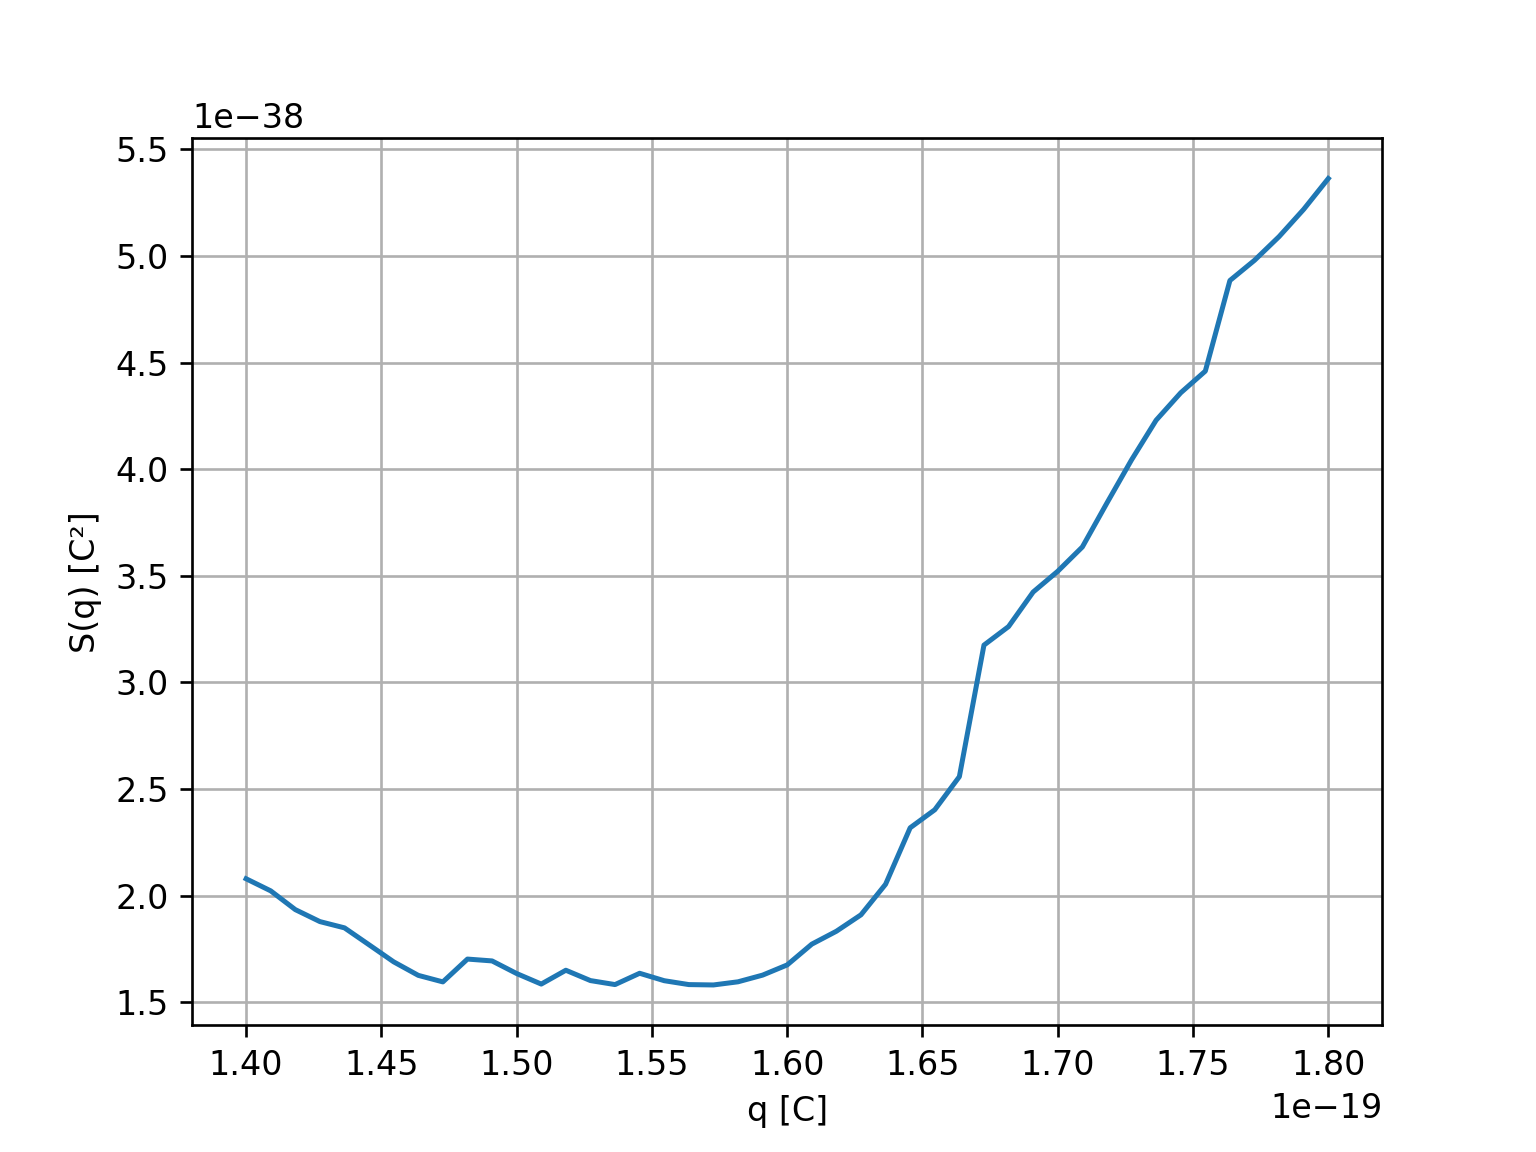
\includegraphics[width=0.50\textwidth]{analysis/graph.png}
        \caption{Grafico della funzione $S(q)$.}
        \label{graph}
    \end{figure}    
    L'espressione analitica di $q_e$ risulta dunque essere:
    \begin{equation}
        \label{qe}
        q_e = \frac{1}{N} \sum_{n=1}^{N} \frac{Q_i}{k_i}
    \end{equation}
    Al valore di $q_e$ sono state attribuite due componenti di errore: una statistica $\sigma_{\text{stat}}$ e una sistematica $\sigma_{\text{sist}}$. La componente statistica è stata determinata mediante deviazione standard della media dei valori ottenuti tramite la \ref{qe}:
    \begin{equation}
        \label{sigma-stat}
        \sigma_{\text{stat}} = \sqrt{ \frac{S(q_e)}{N \left(N-1 \right)} } = 1.26 \cdot 10^{-21} \, \text{C}
    \end{equation}
    La componente sistematica dell'errore è stata determinata mediante propagazione degli errori sulle $Q_i$ nella \ref{qe}:
    \begin{equation}
        \sigma_{\text{sist}} = \frac{1}{N} \sqrt{\sum_{n=1}^{N} \left(\frac{\sigma_{Q_i}}{k_i} \right)^2} = 4.71 \cdot 10^{-23} \, \text{C}
    \end{equation}
    Dalla somma in quadratura delle due componenti di errore, si ottiene l'incertezza su $q_e$.

    \section{Conclusioni}
    Il valore finale per la carica dell'elettrone ottenuto è:
    \begin{equation}
        q_e = \left( 1.57 \pm 0.01 \right) \cdot 10^{-19} \, \text{C}
    \end{equation}
    Tale valore è situato entro $2.33\sigma$ dal valore atteso $e = 1.602176634 \cdot 10^{-19} \, \text{C}$, dunque risulta compatibile. Il discostamento del valore ottenuto dal valore atteso è principalmente determinato dalla poco oculata scelta delle gocce osservate: in particolare, si sono scelte gocce con tempi di caduta eccessivamente ridotti, e/o interagenti con altre gocce. Il primo fattore ha influito sulle misurazioni degli intervalli di tempo $t$, poiché con tempi di caduta minori l'errore percentuale diventa maggiore. Il secondo fattore, invece, può aver provocato scambi di cariche tra gocce o confusione nello sperimentatore, il quale può aver effettuato misure su gocce differenti.
    
    \newpage

    \section*{Appendice}

    \begin{table}[H]
        \centering
        \begin{tabular}{||c|c|c||}
            \hline
            $t \pm \sigma_t \, \left[\text{s}\right]$ & $v_0 \, \left[\mu\text{m/s}\right]$ & $r \pm \sigma_r \, \left[\mu\text{m}\right]$ \\\hline
            \hline
            $61.4 \pm 0.5$ & $8.14$ & $0.245 \pm 0.001$ \\\hline
            $64.3 \pm 0.5$ & $7.78$ & $0.238 \pm 0.001$ \\\hline
            $48.0 \pm 0.5$ & $1.04$ & $0.281 \pm 0.002$ \\\hline
            $53.3 \pm 0.5$ & $9.38$ & $0.265 \pm 0.001$ \\\hline
            $81.6 \pm 0.5$ & $6.13$ & $0.208 \pm 0.008$ \\\hline
            \hline
            $t \pm \sigma_t \, \left[\text{s}\right]$ & $v_E \, \left[\mu\text{m/s}\right]$ & $Q \pm \sigma_Q \, \left[\cdot 10^{-19} \text{C}\right]$ \\\hline
            \hline
            $1.4 \pm 0.5$ & $357$ & $3.6 \pm 1.3\,\ast$ \\\hline
            $1.0 \pm 0.5$ & $500$ & $5.1 \pm 2.6\,\ast$ \\\hline
            $1.3 \pm 0.5$ & $385$ & $3.9 \pm 1.5$ \\\hline
            $1.3 \pm 0.5$ & $385$ & $3.9 \pm 1.5$ \\\hline
            $1.2 \pm 0.5$ & $417$ & $4.3 \pm 1.8\,\ast$ \\\hline
            \hline
            $t \pm \sigma_t \, \left[\text{s}\right]$ & $v_E \, \left[\mu\text{m/s}\right]$ & $Q \pm \sigma_Q \, \left[\cdot 10^{-19} \text{C}\right]$ \\\hline
            \hline
            $3.3 \pm 0.5$ & $152$ & $1.7 \pm 0.3\,\ast$ \\\hline
            $1.0 \pm 0.5$ & $500$ & $5.3 \pm 2.7\,\ast$ \\\hline
            $0.9 \pm 0.5$ & $556$ & $5.9 \pm 3.3\,\ast$ \\\hline
            $1.3 \pm 0.5$ & $385$ & $4.1 \pm 1.6\,\ast$ \\\hline
            $1.1 \pm 0.5$ & $455$ & $4.8 \pm 2.2\,\ast$ \\\hline
        \end{tabular}
        \caption{Goccia 1 $\left(T = 21.5\, \text{°C}\right)$ con $\Delta V = 0,+394,-394 \,\text{V}$.}
        \label{goccia-1}
    \end{table}

    \begin{table}[H]
        \centering
        \begin{tabular}{||c|c|c||}
            \hline
            $t \pm \sigma_t \, \left[\text{s}\right]$ & $v_0 \, \left[\mu\text{m/s}\right]$ & $r \pm \sigma_r \, \left[\mu\text{m}\right]$ \\\hline
            \hline
            $20.4 \pm 0.5$ & $24.5$ & $0.451 \pm 0.006$ \\\hline
            $23.6 \pm 0.5$ & $21.2$ & $0.417 \pm 0.005$ \\\hline
            $22.2 \pm 0.5$ & $22.5$ & $0.431 \pm 0.005$ \\\hline
            $24.5 \pm 0.5$ & $20.4$ & $0.408 \pm 0.005$ \\\hline
            $19.5 \pm 0.5$ & $25.6$ & $0.462 \pm 0.006$ \\\hline
            \hline
            $t \pm \sigma_t \, \left[\text{s}\right]$ & $v_E \, \left[\mu\text{m/s}\right]$ & $Q \pm \sigma_Q \, \left[\cdot 10^{-19} \text{C}\right]$ \\\hline
            \hline
            $6.0 \pm 0.5$ & $83$ & $1.4 \pm 0.2\,\ast$ \\\hline
            $5.5 \pm 0.5$ & $91$ & $1.6 \pm 0.2$ \\\hline
            $5.5 \pm 0.5$ & $91$ & $1.6 \pm 0.2$ \\\hline
            $5.5 \pm 0.5$ & $91$ & $1.6 \pm 0.2$ \\\hline
            $5.6 \pm 0.5$ & $89$ & $1.6 \pm 0.2$ \\\hline
            \hline
            $t \pm \sigma_t \, \left[\text{s}\right]$ & $v_E \, \left[\mu\text{m/s}\right]$ & $Q \pm \sigma_Q \, \left[\cdot 10^{-19} \text{C}\right]$ \\\hline
            \hline
            $ 9.7 \pm 0.5$ & $52$ & $1.7 \pm 0.2$ \\\hline
            $ 9.8 \pm 0.5$ & $51$ & $1.7 \pm 0.2$ \\\hline
            $10.6 \pm 0.5$ & $47$ & $1.6 \pm 0.2\,\ast$ \\\hline
            $12.3 \pm 0.5$ & $41$ & $1.5 \pm 0.1\,\ast$ \\\hline
            $10.1 \pm 0.5$ & $50$ & $1.7 \pm 0.2$ \\\hline
        \end{tabular}
        \caption{Goccia 2 $\left(T = 21.5\, \text{°C}\right)$ con $\Delta V = 0,+395,-395 \,\text{V}$.}
        \label{goccia-2}
    \end{table}

    \begin{table}[H]
        \centering
        \begin{tabular}{||c|c|c||}
            \hline
            $t \pm \sigma_t \, \left[\text{s}\right]$ & $v_0 \, \left[\mu\text{m/s}\right]$ & $r \pm \sigma_r \, \left[\mu\text{m}\right]$ \\\hline
            \hline
            $37.4 \pm 0.5$ & $13.4$ & $0.323 \pm 0.002$ \\\hline
            $44.3 \pm 0.5$ & $11.3$ & $0.294 \pm 0.002$ \\\hline
            $41.1 \pm 0.5$ & $12.2$ & $0.307 \pm 0.002$ \\\hline
            $38.8 \pm 0.5$ & $12.9$ & $0.317 \pm 0.002$ \\\hline
            $38.6 \pm 0.5$ & $13.0$ & $0.318 \pm 0.002$ \\\hline
            \hline
            $t \pm \sigma_t \, \left[\text{s}\right]$ & $v_E \, \left[\mu\text{m/s}\right]$ & $Q \pm \sigma_Q \, \left[\cdot 10^{-19} \text{C}\right]$ \\\hline
            \hline
            $1.3 \pm 0.5$ & $385$ & $6.0 \pm 2.4\,\ast$ \\\hline
            $1.2 \pm 0.5$ & $417$ & $6.5 \pm 2.8\,\ast$ \\\hline
            $1.9 \pm 0.5$ & $263$ & $4.1 \pm 1.1\,\ast$ \\\hline
            $1.6 \pm 0.5$ & $313$ & $4.9 \pm 1.6\,\ast$ \\\hline
            $1.5 \pm 0.5$ & $333$ & $5.2 \pm 1.8\,\ast$ \\\hline
            \hline
            $t \pm \sigma_t \, \left[\text{s}\right]$ & $v_E \, \left[\mu\text{m/s}\right]$ & $Q \pm \sigma_Q \, \left[\cdot 10^{-19} \text{C}\right]$ \\\hline
            \hline
            $1.1 \pm 0.5$ & $455$ & $7.6 \pm 3.5\,\ast$ \\\hline
            $1.5 \pm 0.5$ & $333$ & $5.6 \pm 1.9\,\ast$ \\\hline
            $1.7 \pm 0.5$ & $294$ & $5.0 \pm 1.5\,\ast$ \\\hline
            $1.6 \pm 0.5$ & $313$ & $5.3 \pm 1.7$ \\\hline
            $1.6 \pm 0.5$ & $313$ & $5.3 \pm 1.7$ \\\hline
        \end{tabular}
        \caption{Goccia 3 $\left(T = 21.5\, \text{°C}\right)$ con $\Delta V = 0,+395,-395 \,\text{V}$.}
        \label{goccia-3}
    \end{table}

    \begin{table}[H]
        \centering
        \begin{tabular}{||c|c|c||}
            \hline
            $t \pm \sigma_t \, \left[\text{s}\right]$ & $v_0 \, \left[\mu\text{m/s}\right]$ & $r \pm \sigma_r \, \left[\mu\text{m}\right]$ \\\hline
            \hline
            $48.5 \pm 0.5$ & $10.3$ & $0.280 \pm 0.002$ \\\hline
            $65.0 \pm 0.5$ & $7.69$ & $0.237 \pm 0.001$ \\\hline
            $69.5 \pm 0.5$ & $7.19$ & $0.228 \pm 0.001$ \\\hline
            $39.1 \pm 0.5$ & $12.8$ & $0.316 \pm 0.002$ \\\hline
            $46.4 \pm 0.5$ & $10.8$ & $0.287 \pm 0.002$ \\\hline
            \hline
            $t \pm \sigma_t \, \left[\text{s}\right]$ & $v_E \, \left[\mu\text{m/s}\right]$ & $Q \pm \sigma_Q \, \left[\cdot 10^{-19} \text{C}\right]$ \\\hline
            \hline
            $1.3 \pm 0.5$ & $385$ & $4.1 \pm 1.6$ \\\hline
            $1.1 \pm 0.5$ & $455$ & $4.9 \pm 2.3\,\ast$ \\\hline
            $1.4 \pm 0.5$ & $357$ & $3.8 \pm 1.4\,\ast$ \\\hline
            $1.3 \pm 0.5$ & $385$ & $4.1 \pm 1.6$ \\\hline
            $1.3 \pm 0.5$ & $385$ & $4.1 \pm 1.6$ \\\hline
            \hline
            $t \pm \sigma_t \, \left[\text{s}\right]$ & $v_E \, \left[\mu\text{m/s}\right]$ & $Q \pm \sigma_Q \, \left[\cdot 10^{-19} \text{C}\right]$ \\\hline
            \hline
            $1.2 \pm 0.5$ & $417$ & $4.7 \pm 2.0\,\ast$ \\\hline
            $1.3 \pm 0.5$ & $385$ & $4.3 \pm 1.7\,\ast$ \\\hline
            $1.0 \pm 0.5$ & $500$ & $5.6 \pm 2.9\,\ast$ \\\hline
            $1.4 \pm 0.5$ & $357$ & $4.0 \pm 1.5\,\ast$ \\\hline
            $1.2 \pm 0.5$ & $417$ & $4.7 \pm 2.0\,\ast$ \\\hline
        \end{tabular}
        \caption{Goccia 4 $\left(T = 22.0\, \text{°C}\right)$ con $\Delta V = 0,+396,-396 \,\text{V}$.}
        \label{goccia-4}
    \end{table}

    \begin{table}[H]
        \centering
        \begin{tabular}{||c|c|c||}
            \hline
            $t \pm \sigma_t \, \left[\text{s}\right]$ & $v_0 \, \left[\mu\text{m/s}\right]$ & $r \pm \sigma_r \, \left[\mu\text{m}\right]$ \\\hline
            \hline
            $59.2 \pm 0.5$ & $8.45$ & $0.250 \pm 0.001$ \\\hline
            $40.9 \pm 0.5$ & $12.2$ & $0.308 \pm 0.002$ \\\hline
            $59.8 \pm 0.5$ & $8.36$ & $0.249 \pm 0.001$ \\\hline
            $59.9 \pm 0.5$ & $8.35$ & $0.248 \pm 0.001$ \\\hline
            $55.3 \pm 0.5$ & $9.04$ & $0.260 \pm 0.001$ \\\hline
            \hline
            $t \pm \sigma_t \, \left[\text{s}\right]$ & $v_E \, \left[\mu\text{m/s}\right]$ & $Q \pm \sigma_Q \, \left[\cdot 10^{-19} \text{C}\right]$ \\\hline
            \hline
            $2.0 \pm 0.5$ & $250$ & $3.0 \pm 0.8$ \\\hline
            $1.9 \pm 0.5$ & $263$ & $3.1 \pm 0.8\,\ast$ \\\hline
            $2.1 \pm 0.5$ & $238$ & $2.8 \pm 0.7\,\ast$ \\\hline
            $1.7 \pm 0.5$ & $294$ & $3.5 \pm 1.1\,\ast$ \\\hline
            $2.2 \pm 0.5$ & $227$ & $2.7 \pm 0.6\,\ast$ \\\hline
            \hline
            $t \pm \sigma_t \, \left[\text{s}\right]$ & $v_E \, \left[\mu\text{m/s}\right]$ & $Q \pm \sigma_Q \, \left[\cdot 10^{-19} \text{C}\right]$ \\\hline
            \hline
            $2.1 \pm 0.5$ & $238$ & $3.0 \pm 0.8$ \\\hline
            $2.0 \pm 0.5$ & $250$ & $3.2 \pm 0.8\,\ast$ \\\hline
            $2.3 \pm 0.5$ & $217$ & $2.8 \pm 0.6\,\ast$ \\\hline
            $1.8 \pm 0.5$ & $278$ & $3.5 \pm 1.0\,\ast$ \\\hline
            $2.1 \pm 0.5$ & $238$ & $3.0 \pm 0.8$ \\\hline
        \end{tabular}
        \caption{Goccia 5 $\left(T = 22.0\, \text{°C}\right)$ con $\Delta V = 0,+396,-396 \,\text{V}$.}
        \label{goccia-5}
    \end{table}

    \begin{table}[H]
        \centering
        \begin{tabular}{||c|c|c||}
            \hline
            $t \pm \sigma_t \, \left[\text{s}\right]$ & $v_0 \, \left[\mu\text{m/s}\right]$ & $r \pm \sigma_r \, \left[\mu\text{m}\right]$ \\\hline
            \hline
            $53.6 \pm 0.5$ & $9.33$ & $0.265 \pm 0.001$ \\\hline
            $52.4 \pm 0.5$ & $9.54$ & $0.268 \pm 0.001$ \\\hline
            $48.0 \pm 0.5$ & $10.4$ & $0.282 \pm 0.002$ \\\hline
            $49.2 \pm 0.5$ & $10.2$ & $0.278 \pm 0.002$ \\\hline
            $50.8 \pm 0.5$ & $9.84$ & $0.273 \pm 0.002$ \\\hline
            \hline
            $t \pm \sigma_t \, \left[\text{s}\right]$ & $v_E \, \left[\mu\text{m/s}\right]$ & $Q \pm \sigma_Q \, \left[\cdot 10^{-19} \text{C}\right]$ \\\hline
            \hline
            $2.3 \pm 0.5$ & $217$ & $2.9 \pm 0.7\,\ast$ \\\hline
            $2.7 \pm 0.5$ & $185$ & $2.4 \pm 0.5\,\ast$ \\\hline
            $2.5 \pm 0.5$ & $200$ & $2.6 \pm 0.6\,\ast$ \\\hline
            $2.4 \pm 0.5$ & $208$ & $2.8 \pm 0.6$ \\\hline
            $2.4 \pm 0.5$ & $208$ & $2.8 \pm 0.6$ \\\hline
            \hline
            $t \pm \sigma_t \, \left[\text{s}\right]$ & $v_E \, \left[\mu\text{m/s}\right]$ & $Q \pm \sigma_Q \, \left[\cdot 10^{-19} \text{C}\right]$ \\\hline
            \hline
            $2.2 \pm 0.5$ & $227$ & $3.3 \pm 0.8\,\ast$ \\\hline
            $2.4 \pm 0.5$ & $208$ & $3.0 \pm 0.7$ \\\hline
            $2.3 \pm 0.5$ & $217$ & $3.2 \pm 0.7\,\ast$ \\\hline
            $2.5 \pm 0.5$ & $200$ & $2.9 \pm 0.6\,\ast$ \\\hline
            $2.4 \pm 0.5$ & $208$ & $3.0 \pm 0.7$ \\\hline
        \end{tabular}
        \caption{Goccia 6 $\left(T = 22.0\, \text{°C}\right)$ con $\Delta V = 0,+396,-396 \,\text{V}$.}
        \label{goccia-6}
    \end{table}

    \begin{table}[H]
        \centering
        \begin{tabular}{||c|c|c||}
            \hline
            $t \pm \sigma_t \, \left[\text{s}\right]$ & $v_0 \, \left[\mu\text{m/s}\right]$ & $r \pm \sigma_r \, \left[\mu\text{m}\right]$ \\\hline
            \hline
            $50.2 \pm 0.5$ & $9.96$ & $0.275 \pm 0.002$ \\\hline
            $61.0 \pm 0.5$ & $8.20$ & $0.246 \pm 0.001$ \\\hline
            $69.0 \pm 0.5$ & $7.25$ & $0.229 \pm 0.001$ \\\hline
            $71.8 \pm 0.5$ & $6.96$ & $0.224 \pm 0.001$ \\\hline
            $61.4 \pm 0.5$ & $8.14$ & $0.245 \pm 0.001$ \\\hline
            \hline
            $t \pm \sigma_t \, \left[\text{s}\right]$ & $v_E \, \left[\mu\text{m/s}\right]$ & $Q \pm \sigma_Q \, \left[\cdot 10^{-19} \text{C}\right]$ \\\hline
            \hline
            $1.2 \pm 0.5$ & $417$ & $4.6 \pm 2.0\,\ast$ \\\hline
            $1.0 \pm 0.5$ & $500$ & $5.6 \pm 2.8$ \\\hline
            $0.9 \pm 0.5$ & $556$ & $6.2 \pm 3.5\,\ast$ \\\hline
            $1.1 \pm 0.5$ & $455$ & $5.0 \pm 2.3\,\ast$ \\\hline
            $1.0 \pm 0.5$ & $500$ & $5.6 \pm 2.8$ \\\hline
            \hline
            $t \pm \sigma_t \, \left[\text{s}\right]$ & $v_E \, \left[\mu\text{m/s}\right]$ & $Q \pm \sigma_Q \, \left[\cdot 10^{-19} \text{C}\right]$ \\\hline
            \hline
            $1.3 \pm 0.5$ & $385$ & $4.4 \pm 1.7\,\ast$ \\\hline
            $1.4 \pm 0.5$ & $357$ & $4.1 \pm 1.5\,\ast$ \\\hline
            $1.2 \pm 0.5$ & $417$ & $4.8 \pm 2.0\,\ast$ \\\hline
            $0.9 \pm 0.5$ & $556$ & $6.4 \pm 3.6\,\ast$ \\\hline
            $1.0 \pm 0.5$ & $500$ & $5.7 \pm 2.9\,\ast$ \\\hline
        \end{tabular}
        \caption{Goccia 7 $\left(T = 22.0\, \text{°C}\right)$ con $\Delta V = 0,+396,-396 \,\text{V}$.}
        \label{goccia-7}
    \end{table}

    \begin{table}[H]
        \centering
        \begin{tabular}{||c|c|c||}
            \hline
            $t \pm \sigma_t \, \left[\text{s}\right]$ & $v_0 \, \left[\mu\text{m/s}\right]$ & $r \pm \sigma_r \, \left[\mu\text{m}\right]$ \\\hline
            \hline
            $15.9 \pm 0.5$ & $31.4$ & $0.516 \pm 0.009$ \\\hline
            $15.4 \pm 0.5$ & $32.5$ & $0.525 \pm 0.009$ \\\hline
            $17.3 \pm 0.5$ & $28.9$ & $0.493 \pm 0.008$ \\\hline
            $16.0 \pm 0.5$ & $31.3$ & $0.514 \pm 0.009$ \\\hline
            $17.8 \pm 0.5$ & $28.1$ & $0.486 \pm 0.007$ \\\hline
            \hline
            $t \pm \sigma_t \, \left[\text{s}\right]$ & $v_E \, \left[\mu\text{m/s}\right]$ & $Q \pm \sigma_Q \, \left[\cdot 10^{-19} \text{C}\right]$ \\\hline
            \hline
            $1.9 \pm 0.5$ & $263$ & $6.7 \pm 2.0$ \\\hline
            $1.9 \pm 0.5$ & $263$ & $6.7 \pm 2.0$ \\\hline
            $1.7 \pm 0.5$ & $294$ & $7.6 \pm 2.5\,\ast$ \\\hline
            $1.7 \pm 0.5$ & $294$ & $7.6 \pm 2.5\,\ast$ \\\hline
            $1.5 \pm 0.5$ & $333$ & $8.7 \pm 3.2\,\ast$ \\\hline
            \hline
            $t \pm \sigma_t \, \left[\text{s}\right]$ & $v_E \, \left[\mu\text{m/s}\right]$ & $Q \pm \sigma_Q \, \left[\cdot 10^{-19} \text{C}\right]$ \\\hline
            \hline
            $2.0 \pm 0.5$ & $250$ & $8.0 \pm 2.3\,\ast$ \\\hline
            $2.3 \pm 0.5$ & $217$ & $7.1 \pm 1.8\,\ast$ \\\hline
            $2.1 \pm 0.5$ & $238$ & $7.7 \pm 2.1\,\ast$ \\\hline
            $2.5 \pm 0.5$ & $200$ & $6.6 \pm 1.6\,\ast$ \\\hline
            $2.2 \pm 0.5$ & $227$ & $7.4 \pm 1.9\,\ast$ \\\hline
        \end{tabular}
        \caption{Goccia 8 $\left(T = 22.0\, \text{°C}\right)$ con $\Delta V = 0,+396,-396 \,\text{V}$.}
        \label{goccia-8}
    \end{table}

    \begin{table}[H]
        \centering
        \begin{tabular}{||c|c|c||}
            \hline
            $t \pm \sigma_t \, \left[\text{s}\right]$ & $v_0 \, \left[\mu\text{m/s}\right]$ & $r \pm \sigma_r \, \left[\mu\text{m}\right]$ \\\hline
            \hline
            $32.7 \pm 0.5$ & $15.3$ & $0.349 \pm 0.003$ \\\hline
            $37.3 \pm 0.5$ & $13.4$ & $0.324 \pm 0.002$ \\\hline
            $31.1 \pm 0.5$ & $16.1$ & $0.358 \pm 0.003$ \\\hline
            $37.8 \pm 0.5$ & $13.2$ & $0.322 \pm 0.002$ \\\hline
            $32.1 \pm 0.5$ & $15.6$ & $0.352 \pm 0.003$ \\\hline
            \hline
            $t \pm \sigma_t \, \left[\text{s}\right]$ & $v_E \, \left[\mu\text{m/s}\right]$ & $Q \pm \sigma_Q \, \left[\cdot 10^{-19} \text{C}\right]$ \\\hline
            \hline
            $5.0 \pm 0.5$ & $100 $ & $1.5 \pm 0.2\,\ast$ \\\hline
            $5.2 \pm 0.5$ & $96.2$ & $1.4 \pm 0.2\,\ast$ \\\hline
            $5.1 \pm 0.5$ & $98.0$ & $1.5 \pm 0.2\,\ast$ \\\hline
            $5.2 \pm 0.5$ & $96.2$ & $1.4 \pm 0.2\,\ast$ \\\hline
            $5.1 \pm 0.5$ & $98.0$ & $1.5 \pm 0.2\,\ast$ \\\hline
            \hline
            $t \pm \sigma_t \, \left[\text{s}\right]$ & $v_E \, \left[\mu\text{m/s}\right]$ & $Q \pm \sigma_Q \, \left[\cdot 10^{-19} \text{C}\right]$ \\\hline
            \hline
            $8.2 \pm 0.5$ & $61.0$ & $1.3 \pm 0.1\,\ast$ \\\hline
            $7.8 \pm 0.5$ & $64.1$ & $1.4 \pm 0.1\,\ast$ \\\hline
            $7.6 \pm 0.5$ & $65.8$ & $1.4 \pm 0.1\,\ast$ \\\hline
            $7.5 \pm 0.5$ & $66.7$ & $1.4 \pm 0.1\,\ast$ \\\hline
            $7.5 \pm 0.5$ & $66.7$ & $1.4 \pm 0.1\,\ast$ \\\hline
        \end{tabular}
        \caption{Goccia 9 $\left(T = 22.0\, \text{°C}\right)$ con $\Delta V = 0,+396,-396 \,\text{V}$.}
        \label{goccia-9}
    \end{table}

    \begin{table}[H]
        \centering
        \begin{tabular}{||c|c|c||}
            \hline
            $t \pm \sigma_t \, \left[\text{s}\right]$ & $v_0 \, \left[\mu\text{m/s}\right]$ & $r \pm \sigma_r \, \left[\mu\text{m}\right]$ \\\hline
            \hline
            $22.5 \pm 0.5$ & $22.2$ & $0.428 \pm 0.005$ \\\hline
            $23.2 \pm 0.5$ & $21.6$ & $0.421 \pm 0.005$ \\\hline
            $23.5 \pm 0.5$ & $21.3$ & $0.418 \pm 0.005$ \\\hline
            $25.2 \pm 0.5$ & $19.8$ & $0.402 \pm 0.004$ \\\hline
            $24.6 \pm 0.5$ & $20.3$ & $0.408 \pm 0.005$ \\\hline
            \hline
            $t \pm \sigma_t \, \left[\text{s}\right]$ & $v_E \, \left[\mu\text{m/s}\right]$ & $Q \pm \sigma_Q \, \left[\cdot 10^{-19} \text{C}\right]$ \\\hline
            \hline
            $1.4 \pm 0.5$ & $357$ & $7.7 \pm 2.9$ \\\hline
            $1.3 \pm 0.5$ & $385$ & $8.4 \pm 3.4\,\ast$ \\\hline
            $1.4 \pm 0.5$ & $357$ & $7.7 \pm 2.9$ \\\hline
            $1.4 \pm 0.5$ & $357$ & $7.7 \pm 2.9$ \\\hline
            $1.4 \pm 0.5$ & $357$ & $7.7 \pm 2.9$ \\\hline
            \hline
            $t \pm \sigma_t \, \left[\text{s}\right]$ & $v_E \, \left[\mu\text{m/s}\right]$ & $Q \pm \sigma_Q \, \left[\cdot 10^{-19} \text{C}\right]$ \\\hline
            \hline
            $1.8 \pm 0.5$ & $278$ & $6.9 \pm 2.1\,\ast$ \\\hline
            $1.6 \pm 0.5$ & $313$ & $7.7 \pm 2.6$ \\\hline
            $1.6 \pm 0.5$ & $313$ & $7.7 \pm 2.6$ \\\hline
            $1.5 \pm 0.5$ & $333$ & $8.1 \pm 2.9\,\ast$ \\\hline
            $1.6 \pm 0.5$ & $313$ & $7.7 \pm 2.6$ \\\hline
        \end{tabular}
        \caption{Goccia 10 $\left(T = 22.0\, \text{°C}\right)$ con $\Delta V = 0,+396,-396 \,\text{V}$.}
        \label{goccia-10}
    \end{table}

\end{document}